\documentclass[../../main.tex]{subfiles}
\begin{document}

\begin{flushright}
\footnotesize\textit{【自動文字起こし・要確認】}
\end{flushright}

[解] 点Xに対し, $\overrightarrow{OX} = \vec{x}$ とおく. $\vec{a}$ と $\vec{b}$ は一次独立.
\[ \vec{g} = \dfrac{1}{3}(\vec{a} + \vec{b}) \]
\[ \vec{p} = h\vec{a} \]
\[ \vec{q} = k\vec{b} \]
従って, 直線PQ上の点Xは, $t \in \mathbb{R}$ として
\[ \vec{x} = t h\vec{a} + (1-t) k\vec{b} \]
とおける. これがGを通るので,
\[ th = (1-t)k = \dfrac{1}{3} \]
をみたす $t \in \mathbb{R}$ が存在するから, ($h, k \neq 0$ が必要で)
\[ \dfrac{1}{h} + \dfrac{1}{k} = 3 \quad \cdots (i) \]
さらに, $T = hkS \cdots$ ① である. $\alpha = h+k$ とおく. (i)をみたす
$(h, k) (0 < h, k \le 1)$ は右図太線部.
従って, (i)から $hk = \dfrac{1}{3}(h+k) = \dfrac{1}{3}\alpha$ に注意して, 図でこれらが交点を持つ条件から
\[ \dfrac{1}{3}\left(\dfrac{2}{3} + \dfrac{2}{3}\right) \le \dfrac{1}{3}\alpha \le \dfrac{1}{3}\left(1 + \dfrac{1}{2}\right) \]
\[ \dfrac{4}{9} \le \dfrac{1}{3}\alpha \le \dfrac{1}{2} \]
①に代入して
\[ \dfrac{4}{9}S \le T \le \dfrac{1}{2}S \quad \text{\qed} \]

\begin{center}
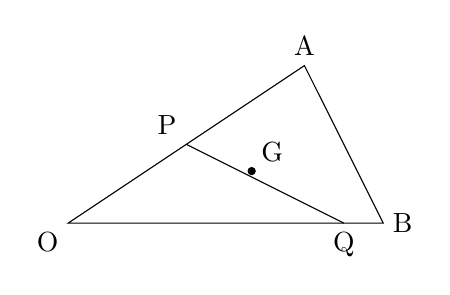
\begin{tikzpicture}
\draw (0,0) node[below left]{O} -- (3,2) node[above]{A} -- (4,0) node[right]{B} -- cycle;
\draw (1.5,1) node[above left]{P};
\draw (3.5,0) node[below]{Q};
\draw (1.5,1) -- (3.5,0);
\node at (2.33,0.66) [above right] {G};
\fill (2.33,0.66) circle (1.5pt);
\end{tikzpicture}
\end{center}

\begin{center}
\begin{tikzpicture}[scale=2]
\draw[->] (-0.2,0) -- (1.5,0) node[right]{$h$};
\draw[->] (0,-0.2) -- (0,1.5) node[above]{$k$};
\draw[dashed] (1/3,-0.2) -- (1/3,1.5);
\draw[domain=0.5:1.2, thick] plot (\x, {\x/(3*\x-1)});
\draw[dashed] (0,1/2) node[left]{$\dfrac{1}{2}$} -- (1,1/2) -- (1,0) node[below]{$1$};
\draw[dashed] (0,1) node[left]{$1$} -- (1/2,1) -- (1/2,0) node[below]{$\dfrac{1}{2}$};
\draw[dashed] (0,2/3) node[left]{$\dfrac{2}{3}$} -- (2/3,2/3) -- (2/3,0) node[below]{$\dfrac{2}{3}$};
\fill (1,1/2) circle (1pt);
\fill (1/2,1) circle (1pt);
\fill (2/3,2/3) circle (1pt);
\node at (1.1, 1.2) {$k = \dfrac{h}{3h-1}$};
\end{tikzpicture}
\end{center}

\end{document}
